% Options for packages loaded elsewhere
\PassOptionsToPackage{unicode}{hyperref}
\PassOptionsToPackage{hyphens}{url}
%
\documentclass[
  12pt,
]{article}
\usepackage{amsmath,amssymb}
\usepackage{iftex}
\ifPDFTeX
  \usepackage[T1]{fontenc}
  \usepackage[utf8]{inputenc}
  \usepackage{textcomp} % provide euro and other symbols
\else % if luatex or xetex
  \usepackage{unicode-math} % this also loads fontspec
  \defaultfontfeatures{Scale=MatchLowercase}
  \defaultfontfeatures[\rmfamily]{Ligatures=TeX,Scale=1}
\fi
\usepackage{lmodern}
\ifPDFTeX\else
  % xetex/luatex font selection
\fi
% Use upquote if available, for straight quotes in verbatim environments
\IfFileExists{upquote.sty}{\usepackage{upquote}}{}
\IfFileExists{microtype.sty}{% use microtype if available
  \usepackage[]{microtype}
  \UseMicrotypeSet[protrusion]{basicmath} % disable protrusion for tt fonts
}{}
\makeatletter
\@ifundefined{KOMAClassName}{% if non-KOMA class
  \IfFileExists{parskip.sty}{%
    \usepackage{parskip}
  }{% else
    \setlength{\parindent}{0pt}
    \setlength{\parskip}{6pt plus 2pt minus 1pt}}
}{% if KOMA class
  \KOMAoptions{parskip=half}}
\makeatother
\usepackage{xcolor}
\usepackage[margin=1in]{geometry}
\usepackage{graphicx}
\makeatletter
\def\maxwidth{\ifdim\Gin@nat@width>\linewidth\linewidth\else\Gin@nat@width\fi}
\def\maxheight{\ifdim\Gin@nat@height>\textheight\textheight\else\Gin@nat@height\fi}
\makeatother
% Scale images if necessary, so that they will not overflow the page
% margins by default, and it is still possible to overwrite the defaults
% using explicit options in \includegraphics[width, height, ...]{}
\setkeys{Gin}{width=\maxwidth,height=\maxheight,keepaspectratio}
% Set default figure placement to htbp
\makeatletter
\def\fps@figure{htbp}
\makeatother
\setlength{\emergencystretch}{3em} % prevent overfull lines
\providecommand{\tightlist}{%
  \setlength{\itemsep}{0pt}\setlength{\parskip}{0pt}}
\setcounter{secnumdepth}{5}
% definitions for citeproc citations
\NewDocumentCommand\citeproctext{}{}
\NewDocumentCommand\citeproc{mm}{%
  \begingroup\def\citeproctext{#2}\cite{#1}\endgroup}
\makeatletter
 % allow citations to break across lines
 \let\@cite@ofmt\@firstofone
 % avoid brackets around text for \cite:
 \def\@biblabel#1{}
 \def\@cite#1#2{{#1\if@tempswa , #2\fi}}
\makeatother
\newlength{\cslhangindent}
\setlength{\cslhangindent}{1.5em}
\newlength{\csllabelwidth}
\setlength{\csllabelwidth}{3em}
\newenvironment{CSLReferences}[2] % #1 hanging-indent, #2 entry-spacing
 {\begin{list}{}{%
  \setlength{\itemindent}{0pt}
  \setlength{\leftmargin}{0pt}
  \setlength{\parsep}{0pt}
  % turn on hanging indent if param 1 is 1
  \ifodd #1
   \setlength{\leftmargin}{\cslhangindent}
   \setlength{\itemindent}{-1\cslhangindent}
  \fi
  % set entry spacing
  \setlength{\itemsep}{#2\baselineskip}}}
 {\end{list}}
\usepackage{calc}
\newcommand{\CSLBlock}[1]{\hfill\break\parbox[t]{\linewidth}{\strut\ignorespaces#1\strut}}
\newcommand{\CSLLeftMargin}[1]{\parbox[t]{\csllabelwidth}{\strut#1\strut}}
\newcommand{\CSLRightInline}[1]{\parbox[t]{\linewidth - \csllabelwidth}{\strut#1\strut}}
\newcommand{\CSLIndent}[1]{\hspace{\cslhangindent}#1}
\RequirePackage{amsthm,amsmath,amsfonts,amssymb}
\RequirePackage[numbers]{natbib}
\RequirePackage{bm}
\RequirePackage{enumerate}
\RequirePackage{enumitem}
\RequirePackage{tabularx}
\RequirePackage{adjustbox}
\RequirePackage{tikz}
\RequirePackage{bbm}
\RequirePackage{lscape}
\RequirePackage{booktabs}
\RequirePackage{longtable}
\RequirePackage{lscape}
\RequirePackage{pifont}
\usepackage{footnote}

\newcommand{\Sc}{\mathcal{S}}
\newcommand{\R}{\mathcal{R}}
\newcommand{\N}{\mathcal{N}}
\newcommand{\X}{\mathcal{X}}
\newcommand{\m}{\mathbf{m}}
\newcommand{\bu}{\mathbf{u}}
\newcommand{\bv}{\mathbf{v}}
\newcommand{\w}{\mathbf{w}}
\newcommand{\x}{\mathbf{x}}
\newcommand{\y}{\mathbf{y}}
\newcommand{\z}{\mathbf{z}}
\newcommand{\bb}{\mathbf{b}}
\newcommand{\brho}{\bm{\rho}}
\newcommand{\bphi}{\bm{\phi}}
\newcommand{\btheta}{\bm{\theta}}
\newcommand{\bpsi}{\bm{\psi}}

\newcommand{\cmark}{\ding{51}}
\newcommand{\xmark}{\ding{55}}

\usepackage{amsmath}
\DeclareMathOperator*{\argmin}{arg\,min}
\ifLuaTeX
  \usepackage{selnolig}  % disable illegal ligatures
\fi
\usepackage{bookmark}
\IfFileExists{xurl.sty}{\usepackage{xurl}}{} % add URL line breaks if available
\urlstyle{same}
\hypersetup{
  pdftitle={Thesis corrections for ``Bayesian spatio-temporal methods for small-area estimation of HIV indicators''},
  hidelinks,
  pdfcreator={LaTeX via pandoc}}

\title{Thesis corrections for ``Bayesian spatio-temporal methods for
small-area estimation of HIV indicators''}
\usepackage{etoolbox}
\makeatletter
\providecommand{\subtitle}[1]{% add subtitle to \maketitle
  \apptocmd{\@title}{\par {\large #1 \par}}{}{}
}
\makeatother
\subtitle{Adam Howes (\texttt{ath19@ic.ac.uk})}
\author{}
\date{\vspace{-2.5em}}

\begin{document}
\maketitle

{
\setcounter{tocdepth}{2}
\tableofcontents
}
\newpage

\section{Dr.~Christopher Paciorek}\label{dr.-christopher-paciorek}

Thank you for the thorough discussion of the thesis. Both during the
defense and in the provided corrections. I have addressed your suggested
corrections point by point, as follows.

\subsection{General comments}\label{general-comments}

\subsubsection{Chapter 4}\label{chapter-4}

\begin{quote}
I'd like to see some more context relating the potential shortcomings to
the public health setting (you have a bit of this in Section 4.1.3). For
a public health analyst, when might they be most concerned about using
the Besag model? What kinds of areal arrangements/neighborhood
structures/types of data might be most prone to concern? E.g., one might
be concerned about cases like Canadian provinces where their populations
are so concentrated right near neighboring US states and most of the
provincial area is sparsely populated.
\end{quote}

In Section 4.1.3. I have modified the text as follows:

``The Besag model was originally proposed by Besag, York, and Mollié
(1991) for use in image analysis. In this setting, areas correspond to
pixels arranged in a regular lattice structure. In an image, the data
point at each pixel can be thought of as an average of the intensity or
colour over the space represented by the pixel.

Since it's original proposal, the Besag model has seen wider use.
However, for small-area estimation of HIV, the spatial structure
corresponds to administrative units. These administrative units may have
a more irregular spatial structure than a lattice. Furthermore, data
points may not come about by uniform averaging over a space. For
example, population density may vary across the area.''

\begin{quote}
And as we discussed, I'd like for you to see if you can drill down into
the localized results of the simulation to give some insight into where
the smoothing is sub-optimal in the simulations. Relatedly would you
expect the features highlighted by your vignettes to occur in reality in
public health settings?*
\end{quote}

Not yet resolved.

\subsubsection{Chapter 5}\label{chapter-5}

\begin{quote}
\emph{I'd like to see the chapter initially clearly lay out the overall
goal, the quantitative representation of that, the various pieces of the
analysis and how they fit together, and the data available, as well as
what components you can estimate uncertainty for. In particular the
notion of ``reaching'' the population needs to be clearly spelled out
initially. And as we discussed, please make clear how prevalence is
needed.}
\end{quote}

I have updated Section 5.1 giving the background for Chapter 5 as
follows:

``In this chapter, I used a Bayesian spatio-temporal model (Section 5.3)
of behavioural data from household surveys (Section 5.2) to estimate HIV
risk group proportions. To then estimate risk group specific HIV
prevalence and HIV incidences (Section 5.4), I combined the proportion
estimates with population size, HIV prevalence and HIV incidence
estimates, as well as risk group specific HIV incidence rate ratios, and
HIV prevalence rate ratios. Finally, by ordering district, age, risk
group strata by HIV incidence, I estimated an upper bound for the number
of new HIV infections that could be averted under different risk
prioritisation strategies (Section 5.4.3).''

\begin{quote}
\emph{Model 5.11 omits various interactions. Focusing on the
category-area-age interaction, which seems like the omitted interaction
most likely to have substantial variation in reality, some effort to
come up with some ``residual'' type diagnostic to assess model
mis-specification in this regard would be helpful (e.g., perhaps some
sort of variogram type analysis of some sort of age-group specific
``working residuals'' to borrow a GLM framing). Or you mentioned fitting
the model with the interaction for one country. If that is not too
burdensome that would also be a reasonable approach here.}
\end{quote}

The linear predictor used for the multinomial logistic regression model
was \[
\eta_{ita} = \theta_{ita} + \beta_k + \zeta_{c[i]k} + \alpha_{ac[i]k} + u_{ik} + \gamma_{tk}.
\] This equation does contain age-country-category interactions
\(\alpha_{ac[i]k}\), but you are right to point out that
age-district-category interactions are omitted. A model containing the
effects \(\alpha_{aik}\) is likely to cause computational difficulties.

\begin{quote}
\emph{The distinct differences between the CPO and information criteria
(IC) results (and the very structured pattern in the surprising IC
results) suggest the possibility of a bug somewhere, as we discussed.
Getting the observation-specific values from INLA might help to better
understand this.}
\end{quote}

I agree.

\subsubsection{Chapter 6}\label{chapter-6}

\begin{quote}
\emph{Chapter 6 extends standard INLA computation in two ways. For the
first, I'd like to see more clarity in how this differs from the
Stringer et al.~(2022) approach (i.e., that you go beyond the Gaussian
mixture over the quadrature points, as we discussed in the defense) and
the details of the software implementation (e.g., giving an overview in
the chapter describing what someone would need to do to make use of your
code/approach).}
\end{quote}

The Stringer, Brown, and Stafford (2022) approach is that of Section
6.1.3.1. It is similar to the \texttt{inla::inla} with
\texttt{method\ =\ "gaussian"}. The novel approach implemented in
Section 6.2 is similar to \texttt{inla::inla} with
\texttt{method\ =\ "laplace"}.

I have clarified this point in the following text: ``First, a
universally applicable implementation of INLA with Laplace marginals,
where automatic differentiation via \texttt{TMB} is used to obtain the
derivatives required for the Laplace approximation. For users of
\texttt{R-INLA}, the Stringer, Brown, and Stafford (2022) approach is
analogous to \texttt{method\ =\ "gaussian"}, while the approach newly
implemented in this chapter is analogous to
\texttt{method\ =\ "laplace"}. Section 6.2 demonstrates the
implementation using two examples, one compatible with \texttt{R-INLA}
and one incompatible.''

\begin{quote}
\emph{As we discussed in the defense, I'm concerned about any case where
one draws from marginals, implicitly assuming no dependence, either at
the hyperparameter level or the latent process level, and then does
inference on a derived quantity that depends on more than one input. You
should be clear anytime you do this that this is problematic (and try to
avoid as much as possible).}
\end{quote}

Not yet resolved.

\begin{quote}
\emph{Relatedly, assuming I'm understanding correctly, there is an
important tradeoff between using Laplace marginals for improved accuracy
for latent marginals and using the Gaussian mixture over the quadrature
points, which allows one to make draws and do inference on any derived
quantity in a way that takes account of posterior dependence between and
amongst hyperparameters and latent process values. If that's the case, I
think it's worth pointing this out and discussing when one can use the
Laplace marginals in a public health context and when one might need to
use the Gaussian mixture.}
\end{quote}

This is an interesting observation. If you're correct, then I agree it
worth pointing out, and it would shift my preference towards using the
mixture of Gaussians approach. The way in which I think that it might
not be correct is that the INLA approach fundamentally targets
marginals, even when using the mixture of Gaussians. That is, the
mixture of Gaussians does not ``take account of posterior dependence
between and amongst hyperparameters and latent process values'' as
suggested. I think this in part because there is work extending INLA to
the joint setting -- which I don't think would need to exist if this
question were correct. To follow up here.

\subsection{Minor comments}\label{minor-comments}

\subsubsection{Chapter 2}\label{chapter-2}

\begin{quote}
\emph{4: ``develop into a stage'' -\textgreater{} ``Infection with HIV
can''}
\end{quote}

Changed to ``If untreated, infection with HIV can develop into a more
advanced stage known as acquired immunodeficiency syndrome (AIDS).''.

\begin{quote}
\emph{6: ``to result a reduction''}
\end{quote}

Changed to ``found complete surgical removal of the foreskin to result
in a reduction''.

\begin{quote}
\emph{11: ``Both DHS and PHIA surveys collecting''}
\end{quote}

Changed to ``Both DHS and PHIA surveys collect demographic, behavioural,
and clinical information.''.

\begin{quote}
\emph{12: individual disclosure: error may come from them not knowing
status}
\end{quote}

Good point, I have added the sentence: ``Furthermore, individuals may be
unaware of their HIV status.''.

\begin{quote}
\emph{14: ``UNAIDS process''}
\end{quote}

Apologies for this stub! This has been been corrected as follows:
``Indeed, careful validation of data by country teams is a crucial part
of the yearly UNAIDS HIV estimates process.''.

\subsubsection{Chapter 3}\label{chapter-3}

\begin{quote}
\emph{16 (and elsewhere): Please look up usage of ``that'' vs.~``which''
so you can join me in the grammar police. ``Models which do not
produce'' -\textgreater{} ``Models that do not produce''}
\end{quote}

Thank you for the pointer, I have fixed this issue and look forward to
joining the good fight.

\begin{quote}
\emph{Fig 3.1: I suggest that you also show the likelihood.}
\end{quote}

I have now included the likelihood in this figure as follows. Figure
6.1, demonstrating the Laplace approximation, has also been updated to
include the likelihood.

\begin{center}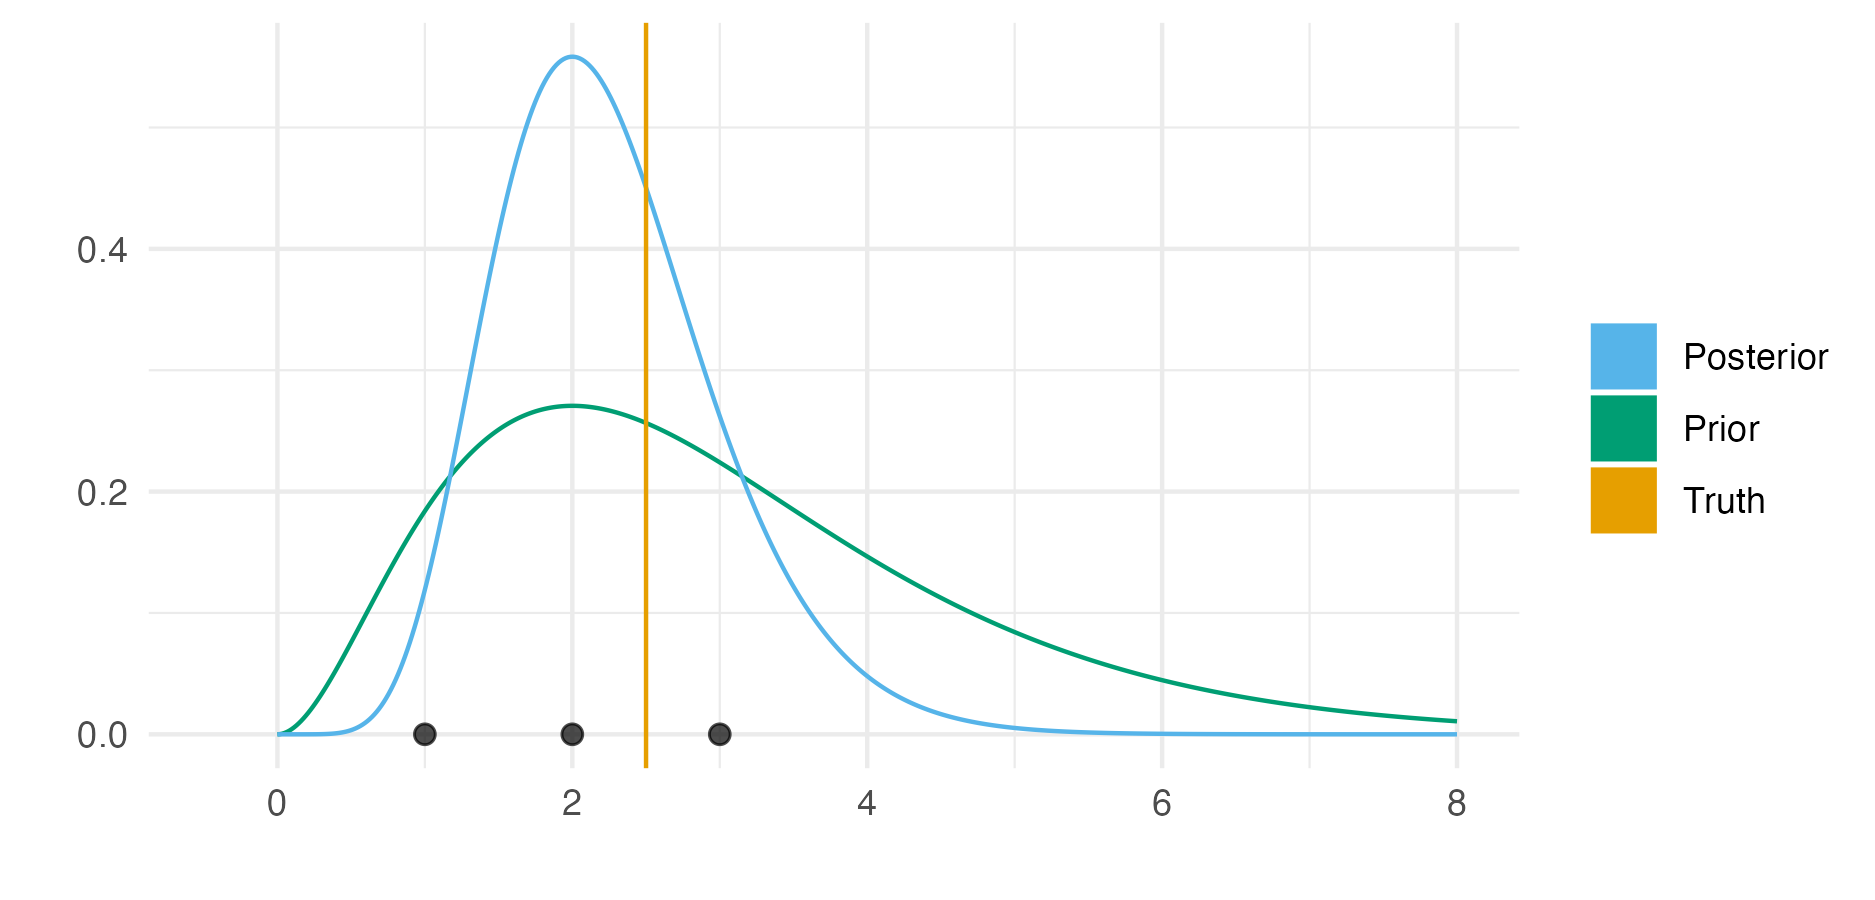
\includegraphics[width=0.95\linewidth]{../figures/bayesian/conjugate} \end{center}

\begin{quote}
\emph{17: Beyond just p(y) even if you know the full form of
p(phi\textbar y) what do you do with it in non-trivial dimensions? You
have to be able to either draw from it or estimate expectations of
interest. the issue is rather broader than just the unknown normalizing
constant.}
\end{quote}

Good point! I have added the sentence: ``Further, even given a closed
form expression for the posterior distribution, if
\(\boldsymbol{\mathbf{\phi}}\) is of moderate to high dimension, then it
is not obvious how to evaluate expressions of interest, which usually
themselves are integrals, or expectations, with respect to the posterior
distribution.''.

\begin{quote}
\emph{19. You haven't defined `convergence' when you dive into
diagnostics.}
\end{quote}

I have altered the text to read: ``After running an MCMC sampler, it is
important that diagnostic checks are used to evaluate whether the Markov
chain has reached its stationary distribution. If so, the Markov chain
is said to have converged, and its samples may be used to compute
posterior quantities. Though it is possible to check poor convergence in
some cases, we may never be sure that a Markov chain has converged, and
thus that results computed from MCMC will be accurate.''.

\begin{quote}
\emph{21. I'd frame this as deterministic approximations need to focus
on approximating expectations of interest. I think of Laplace as
approximating an integral over part of parameter space (often
\textgreater{} random effects') to be able to work with a
smaller-dimensional space, such as for maximization.}
\end{quote}

Thank you for the comment. In Chapter 6, I refer to a Laplace
approximation over part of the parameter space as the marginal Laplace
approximation.

\begin{quote}
\emph{23. ``data is'' -\textgreater{} ``data are'' (also p 66 and
perhaps elsewhere)}
\end{quote}

I have corrected to ``data are'' in this instance and elsewhere in the
thesis.

\begin{quote}
\emph{30. You distinguish ELGM from LGM with having defined eta for LGM
or been explicit about 1:1 relationship of x and y.}
\end{quote}

Good point. In an LGM, it is that there is a one-to-one relationship
between \(\mathbf{y}\) and \(\boldsymbol{\mathbf{\eta}}\). I have added
the sentence: ``In an LGM, like the more general GLMM case as given in
Equation (3.6), there is a one-to-one correspondence between
observations \(y_i\) and elements of the linear predictor \(\eta_i\).''.

\begin{quote}
\emph{Sec 3.4: worth commenting on additivity of these measures that
treat each obs as a unit of information given you are in a spatial
setting.}
\end{quote}

Note connection to SLOO-CV in Chapter 4.

\begin{quote}
\emph{35. (3.30) should be for \(\pi_{2hj}\).}
\end{quote}

Thank you for spotting this! Corrected.

\begin{quote}
\emph{37. ``difficultly''}
\end{quote}

Corrected to ``problem difficulty''.

\begin{quote}
\emph{37. ``arrived at using by''}
\end{quote}

Corrected to ``arrived at by estimating the variance of''.

\subsubsection{Chapter 4}\label{chapter-4-1}

\begin{quote}
\emph{41. Might be worth including the variance piece raised to the
power \texttt{n-c}.}
\end{quote}

I have added the factor \(\tau_u^{\frac{n - n_c}{2}}\). Initially I
excluded this factor as the primary intention of Equation (4.4) is to
demonstrate that \(p(\mathbf{u})\) is a function of the pairwise
differences and thus improper.

\begin{quote}
\emph{41. ``recommended against'': passive, and by who?}
\end{quote}

I have altered the text to read: ``Directly using the Besag model as
described in Section 4.1.1 has several practical limitations in applied
settings. To overcome these limitations, Freni-Sterrantino, Ventrucci,
and Rue (2018) recommend three best practices:''.

\begin{quote}
\emph{42. Why is unit variance correct?}
\end{quote}

Yes that's a good point, what I mean to say is that the singletons have
unit variance in the ``structure matrix'' sense. I have corrected the
text to read that \(p(u_i) \sim \mathcal{N}(0, \tau_u^{-1})\).

\begin{quote}
\emph{47. tau\_v an d tau\_w are not orthogonal - what does this mean?}
\end{quote}

Practically speaking, this means that the posteriors for \(\tau_v\) and
\(\tau_w\) are likely to be correlated. See Figure C.8 and Figure C.9 in
Appendix C for an example, showing that the BYM2 parameterisation
overcomes this issue.

\begin{quote}
\emph{48. Is convolution the right term here?}
\end{quote}

I have altered the text to use the term ``convolved random effects''
following use of this terminology by Morris et al. (2019).

\begin{quote}
\emph{55: what is meant by ``model is implemented in arealutils''?}
\end{quote}

I have updated the text to read: ``in the \texttt{arealutils} R package
(Howes 2023)''.

\begin{quote}
\emph{56: need citation for v being hard to estimate}
\end{quote}

Although I found references (Zhang 2004; Williams and Rasmussen 2006;
Anderes 2010; Karvonen and Oates 2023) supporting difficulties
estimating one or multiple hyperparameters for spatial models (including
using the Matérn kernel) I did not find a reference to directly support
\(\nu\) being difficult to estimate. For example, Williams and Rasmussen
(2006) note that above \(\nu = 7/2\) (i.e.~quite smooth) then it's
difficult to estimate \(\nu\) from ``finite noisy training samples''.
Hence I have updated the text to read: ``We fixed the smoothness
hyperparameter \(\nu\) to \(3/2\) to avoid concerns regarding the joint
identifiability of the smoothness and lengthscale hyperparameters.''.
The observations in Chapter 4 being from a binomial distribution, to me
intuitively, does support further that \(\nu\) would be very difficult
to estimate, but I could be wrong.

\begin{quote}
\emph{56: have Li vary with size?}
\end{quote}

The \(L_i\) did not vary with the size of the area. A fixed number were
used for each area.

\begin{quote}
\emph{56: effect -\textgreater{} affect}
\end{quote}

Change made, thank you!

\begin{quote}
\emph{57: ``and the calibration''}
\end{quote}

I have altered the text to read: ``and the probability integral
transform (PIT; Dawid (1984)) values''.

\begin{quote}
\emph{57: What parameter is shown in Figs 4.7-4.9 - it's not clear
you're assessing the latent process values. And in that case you should
be clear the CRPS is averaged over locations.}
\end{quote}

Not yet resolved.

\begin{quote}
\emph{59: Explain that mean CRPS is mean over the simulations.}
\end{quote}

Not yet resolved.

\begin{quote}
\emph{63: Table 4.4 has no standard errors.}
\end{quote}

Not yet resolved.

\begin{quote}
\emph{64: ``resulted wide''}
\end{quote}

Changed to ``resulted in wide''.

\begin{quote}
\emph{64: surprisingly}
\end{quote}

Changed, thank you!

\begin{quote}
\emph{67: ``This chapter used of area-level models to for point-level
data throughout''. I can't parse this. You can only use point level
model if have point level data.}
\end{quote}

Not yet resolved.

\begin{quote}
\emph{67: ``measures are disaggregated by area'' - not sure of the point
here.}
\end{quote}

Not yet resolved.

\subsubsection{Chapter 5}\label{chapter-5-1}

\begin{quote}
\emph{71: FSW is not defined in Table 1 caption.}
\end{quote}

Changed to ``female sex workers (FSW)''.

\begin{quote}
\emph{71: In Table 1 why does High risk group IRR not vary with local
incidence?}
\end{quote}

The conceptual model underpinning this decision was to frame the
``High'' risk group as a part of the general population at higher risk
and the ``Very High'' risk group as a concentrated epidemic
subpopulation. In reality IRR is likely to vary by local incidence for
the ``Very High'' risk group as well, and as such this is a fair
critique. Practically speaking, the ALPHA network data used to inform
the ``High'' IRR has quite little geographic variation.

\begin{quote}
\emph{71: Purpose of Table 1 is not clear. Nor how IRR is to be used.}
\end{quote}

Not yet resolved.

\begin{quote}
\emph{Tables sometimes appear earlier than they should (e.g., 5.1 and
5.2).}
\end{quote}

Not yet resolved.

\begin{quote}
\emph{77: Table 5.2: phi\_\{ik\} should be u\_\{ik\}.}
\end{quote}

Good spot! Thank you, fixed.

\begin{quote}
\emph{80: Mention country-specific vs single models earlier.}
\end{quote}

Not yet resolved.

\begin{quote}
\emph{82: I would say clearly that model structure for q\_ia is
discussed next.}
\end{quote}

I have altered the text to read: ``As all such surveys occurred in the
years 2013-2018 (Figure 5.2) I assumed no dependence on time, hence
omission of the index \(t\). Model specification for the linear
predictor \(\eta_{ia}\) is discussed in Section 5.3.2.1 to follow.''

\begin{quote}
\emph{85: First paragraph of 5.3.3 is a bit hard to follow.}
\end{quote}

I have altered the text to read: ``Domain experts do not consider having
had sex''in return for gifts, cash or anything else in the past 12
months'' sufficient to constitute sex work. For this reason, I adjusted
the estimates obtained based on the transactional sex survey question to
match alternatively obtained age-country FSW population size estimates.
Taking this approach retained subnational variation informed by the
transactional sex survey question.''.

\begin{quote}
\emph{86: The bio-marker survey data and disaggregation model is
unclear. How are risk groups known for individuals in the survey?}
\end{quote}

Not yet resolved.

\begin{quote}
\emph{88: Section 5.4.3 is hard to understand. I don't understand how it
relates to 5.4.2. ``Reach'' is not clearly defined nor is it clearly
discussed how it is quantified based on the various modeling pieces.}
\end{quote}

Not yet resolved.

\begin{quote}
\emph{91: Not clear what the quantities are in the statement about ``in
most districts adolescent girls aged 15-19 were not sexually active''.
Is this an across-district or within-district quantity?}
\end{quote}

Not yet resolved.

\begin{quote}
\emph{95: does the approach presented allow identification of actual
people or just targeting efforts to reach more such people collectively}
\end{quote}

Not yet resolved.

\begin{quote}
\emph{96: ``Accounting for the 0\% of new infections''?}
\end{quote}

Not yet resolved.

\subsubsection{Chapter 6}\label{chapter-6-1}

\begin{quote}
\emph{106: Not sure what you mean by ``log p(y\textbar x,theta) is
small''. This is the likelihood\ldots{}}
\end{quote}

I based this sentence on Blangiardo et al. (2013).

\begin{quote}
\emph{116: ``in which, which''}
\end{quote}

Changed to ``in which, similar to extended latent Gaussian models''.

\begin{quote}
\emph{122: ``Method'' in Table 6.1 a bit terse.}
\end{quote}

I have updated this column to be more specific about the first word
referring to ``latent field marginals'' and the second being ``over the
hyperparameters'' (apart from for NUTS, which is over the whole space).

\begin{quote}
\emph{122: Is ``Gaussian, EB'' the same as frequentist Laplace approx
(up to hyperparameter prior)? If so, probably worth saying.}
\end{quote}

Yes I believe it is. I have updated the text as follows: ``\ldots{}''.

\begin{quote}
\emph{130: Somewhat unclear how the quadrature is implemented, wrapped
around the TMB-based Laplace approximation. Is your code in R? (Sorry,
this may be because I didn't have time to look through appendices.)}
\end{quote}

Not yet resolved.

\begin{quote}
\emph{131: Using same number of iterations with stan (full posterior,
including latent values) vs tmbstan (hyperparameters, much
lower-dimensional space) seems odd.}
\end{quote}

Here I am using \texttt{tmbstan} with the default option
\texttt{laplace\ =\ FALSE}. Hence the \texttt{tmbstan} sampler is
operating over the full space, just as the \texttt{rstan} sampler. As
such, it's reasonable to use the sample number of iterations with both
samplers.

\begin{quote}
\emph{132: Fig 6.7 is just grid/AGHQ, not EB? If so, why present EB
method?}
\end{quote}

Not yet resolved.

\begin{quote}
\emph{132: Why surprising tmbstan faster than rstan - what are the
different computations involved - having to compute Laplace vs doing HMC
over higher dimensional space. I expect it would vary with I expect it
would vary with hyperparameter and latent dimensions.}
\end{quote}

It is surprising as they are running the same algorithm: HMC over the
full space.

\begin{quote}
\emph{136: ``kridge'' -\textgreater{} ``krige''}
\end{quote}

Changed to \texttt{gstat::krige}.

\begin{quote}
\emph{137: ``this'' in ``this difference'' is unclear.}
\end{quote}

I have altered the text to read: ``As \(\beta_\phi\) was fixed then
differences in approximation accuracy between the Gaussian and Laplace
approximations of \(\phi(s)\) are due only to differences in estimation
of \(u(s)\).''.

\begin{quote}
\emph{143: ``survey weighting increases variance'' - what about effect
of increasing precision in small strata? Are you talking about influence
of complex survey design or somehow about weighting scheme?}
\end{quote}

Not yet resolved.

\begin{quote}
\emph{149: INLA uses CCD for d\textgreater2, right? Would this not work
for this setting?}
\end{quote}

Yes, \texttt{R-INLA} does use central composite design (CCD) for
integration over moderate dimensions. I note that \texttt{R-INLA} uses
CCD for \(m > 2\) in Section 6.1.4.1, illustrate CCD in Figure 6.4, and
mention that it would be of interest to compare PCA-AGHQ to CCD in
Section 6.6.3.1.

\begin{quote}
\emph{151: (6.97) has `d' instead of `m'}
\end{quote}

Agree, fixed swapping \(d\) to \(m\).

\begin{quote}
\emph{154: ``closet''}
\end{quote}

Changed to ``posterior contraction was very close to zero.''.

\begin{quote}
\emph{154: Did you use MAP for theta when looking at Hessian
eigenvalues?}
\end{quote}

Not yet resolved.

\begin{quote}
\emph{156: ``Figure ??''}
\end{quote}

Fixed, thank you.

\begin{quote}
\emph{156: ``far fewer than full 24'' - is this a problem?}
\end{quote}

This is a problem in the sense that it would ideal for the quadrature
nodes used to show some variability in all 24 dimensions. PCA-AGHQ does
improve upon a naive product grid, but is still far from ideal.

\begin{quote}
\emph{156: ``point estimates'' ``distributional quantities'' - need
``and''}
\end{quote}

Fixed, thank you.

\begin{quote}
\emph{157: Need caption to describe the green}
\end{quote}

Thank you, I have updated this caption to read ``The grey histograms
show the 24 hyperparameter marginal distributions obtained with NUTS.
The green lines indicate the position of the 6561 PCA-AGHQ nodes
projected onto each hyperparameter marginal. For some hyperparameters,
the PCA-AGHQ nodes vary over the domain of the posterior marginal
distribution, while for others they concentrate at the mode.''.

\begin{quote}
\emph{165: What went wrong with tmbstan?}
\end{quote}

(Note to self that this is in regard to ``Preliminary testing of this
approach, using \texttt{tmbstan} and setting \texttt{laplace\ =\ TRUE},
did not show immediate success but likely could be worked on.'')

\newpage

\section{Dr.~Adam Sykulski}\label{dr.-adam-sykulski}

Thank you for providing a paper copy of the thesis annotated with
suggested typographical changes. I have made these changes, and
additionally thoroughly proofread the thesis as requested.

\newpage

\section*{References}\label{references}
\addcontentsline{toc}{section}{References}

\phantomsection\label{refs}
\begin{CSLReferences}{1}{0}
\bibitem[\citeproctext]{ref-anderes2010consistent}
Anderes, Ethan. 2010. {``On the Consistent Separation of Scale and
Variance for Gaussian Random Fields.''}

\bibitem[\citeproctext]{ref-besag1991bayesian}
Besag, Julian, Jeremy York, and Annie Mollié. 1991. {``{Bayesian image
restoration, with two applications in spatial statistics}.''}
\emph{Annals of the Institute of Statistical Mathematics} 43 (1): 1--20.

\bibitem[\citeproctext]{ref-blangiardo2013spatial}
Blangiardo, Marta, Michela Cameletti, Gianluca Baio, and Håvard Rue.
2013. {``{Spatial and spatio-temporal models with R-INLA}.''}
\emph{Spatial and Spatio-Temporal Epidemiology} 4: 33--49.

\bibitem[\citeproctext]{ref-dawid1984present}
Dawid, A Philip. 1984. {``{Present position and potential developments:
Some personal views statistical theory the prequential approach}.''}
\emph{Journal of the Royal Statistical Society: Series A (General)} 147
(2): 278--90.

\bibitem[\citeproctext]{ref-freni2018note}
Freni-Sterrantino, Anna, Massimo Ventrucci, and Håvard Rue. 2018. {``{A
note on intrinsic conditional autoregressive models for disconnected
graphs}.''} \emph{Spatial and Spatio-Temporal Epidemiology} 26: 25--34.

\bibitem[\citeproctext]{ref-howes2023arealutils}
Howes, Adam. 2023. \emph{{arealutils: Utility functions for
beyond-borders}}.

\bibitem[\citeproctext]{ref-karvonen2023maximum}
Karvonen, Toni, and Chris J. Oates. 2023. {``Maximum Likelihood
Estimation in Gaussian Process Regression Is Ill-Posed.''} \emph{Journal
of Machine Learning Research} 24 (120): 1--47.
\url{http://jmlr.org/papers/v24/22-1153.html}.

\bibitem[\citeproctext]{ref-morris2019bayesian}
Morris, Mitzi, Katherine Wheeler-Martin, Dan Simpson, Stephen J. Mooney,
Andrew Gelman, and Charles DiMaggio. 2019. {``{Bayesian hierarchical
spatial models: Implementing the Besag York Mollié model in stan}.''}
\emph{Spatial and Spatio-Temporal Epidemiology} 31: 100301.
https://doi.org/\url{https://doi.org/10.1016/j.sste.2019.100301}.

\bibitem[\citeproctext]{ref-stringer2022fast}
Stringer, Alex, Patrick Brown, and Jamie Stafford. 2022. {``{Fast,
scalable approximations to posterior distributions in extended latent
Gaussian models}.''} \emph{Journal of Computational and Graphical
Statistics}, 1--15.

\bibitem[\citeproctext]{ref-williams2006gaussian}
Williams, Christopher KI, and Carl Edward Rasmussen. 2006.
\emph{Gaussian Processes for Machine Learning}. Vol. 2. 3. MIT press
Cambridge, MA.

\bibitem[\citeproctext]{ref-zhang2004inconsistent}
Zhang, Hao. 2004. {``Inconsistent Estimation and Asymptotically Equal
Interpolations in Model-Based Geostatistics.''} \emph{Journal of the
American Statistical Association} 99 (465): 250--61.

\end{CSLReferences}

\end{document}
